%!TEX root = ../../Main.tex
\graphicspath{{Chapters/SystemArkitektur/}}
%-------------------------------------------------------------------------------

\section{System Arkitektur}

Systemarkitekturen i projektet har været en iterativ proces og er derfor blevet rekonstrueret og ændret undervejs i projekt-forløbet.
Arkitekturen i systemet danner rammer for, hvordan BA-TA's logiske system er opbygget og implementeret. Hermed dannes der et overblik over den logiske funktionalitet og hvordan den bruges på tværs af de forskellige drivere i systemet.

\subsection{Entity Relationship Diagram}
På nedenstående figur, \ref{fig:Entity}, danner der et overblik over den logiske funktionalitet på tværs af systemet, som er udmundet i funktioner i de forskellige driver-klasser.

\begin{figure}[H]
	\centering
	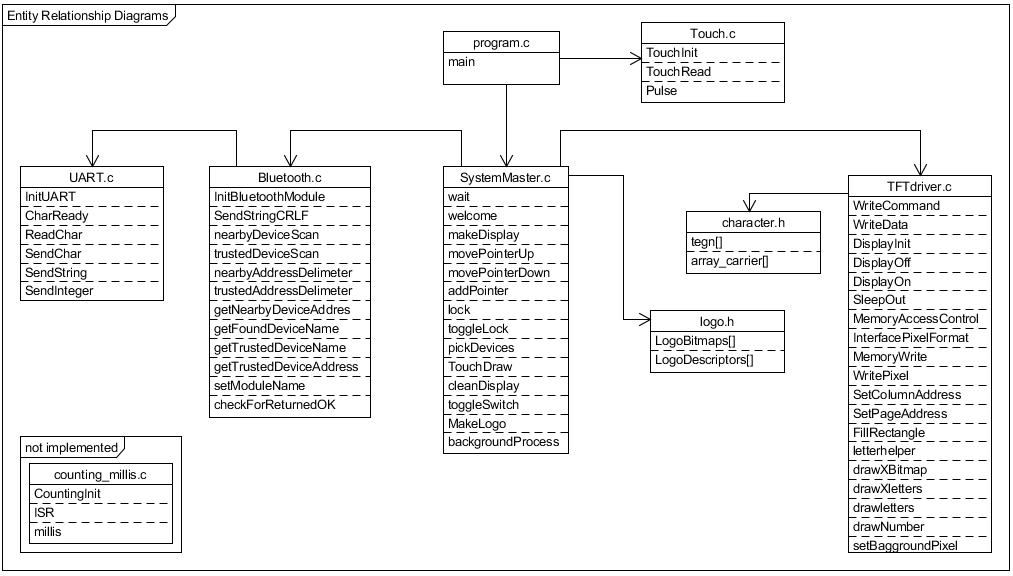
\includegraphics[width = 500 pt]{Img/Entity.png}
	\caption{Entity Relationship Diagrams}
	\label{fig:Entity}
\end{figure}

\newpage

\subsection{Sekvensdiagrammer}
Da der hermed er dannet et overordnet overblik af systemets logiske funktionalitet, kan der dermed refereres til den logiske implementering af projektets tre Use Cases. Hvert respektive sekvensdiagram tager udgangspunkt i det respektive samme nummer af Use Case. Hermed er Sekvens Diagram 1 relateret til Use Case 1, Sekvens Diagram 2 til Use Case 2 og så videre.

For besparelse tekst fylde i diagrammerne og dermed også for overskuelighedens skyld, er Bluetooth nævnt i diagrammerne som forkortelsen "BT".

\hfill \break
\hfill \break

\begin{figure}[H]
	\centering
	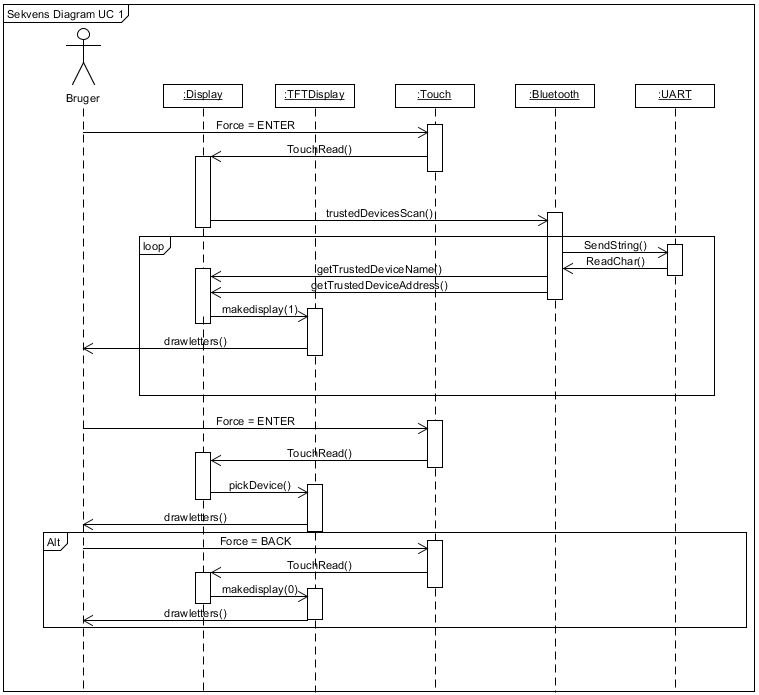
\includegraphics[width = 400 pt]{Img/SD1.png}
	\caption{Sekvensdiagram for Use Case 1}
	\label{fig:SD1}
\end{figure}

\hfill \break
\hfill \break
\hfill \break
\hfill \break
\hfill \break
\hfill \break
\hfill \break
\hfill \break

\begin{figure}[H]
	\centering
	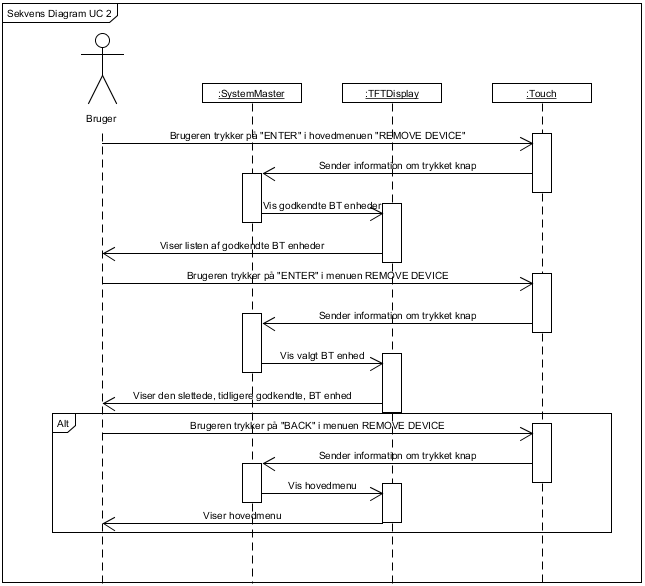
\includegraphics[width = 400 pt]{Img/SD2.png}
	\caption{Sekvensdiagram for Use Case 2}
	\label{fig:SD2}
\end{figure}

\hfill \break
\hfill \break
\hfill \break
\hfill \break
\hfill \break
\hfill \break
\hfill \break
\hfill \break
\hfill \break
\hfill \break
\hfill \break
\hfill \break
\hfill \break
\hfill \break
\hfill \break
\hfill \break
\hfill \break


\begin{figure}[H]
	\centering
	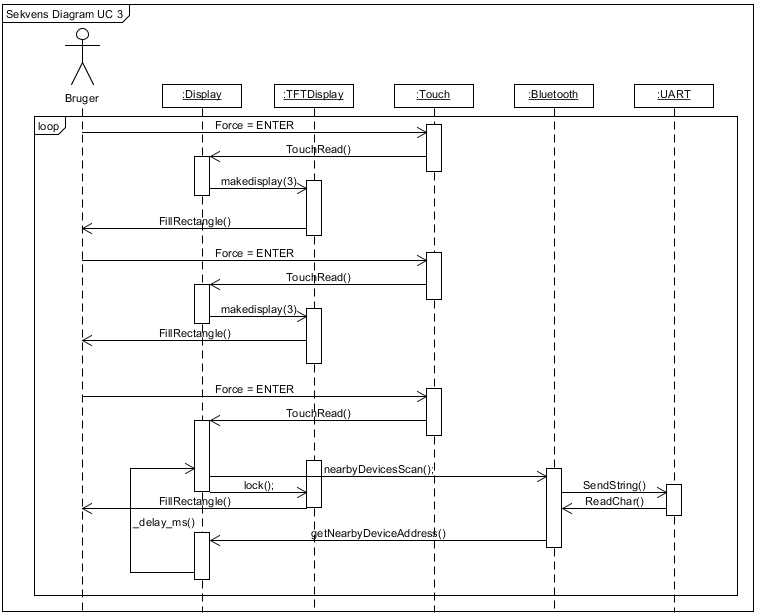
\includegraphics[width = 400 pt]{Img/SD3.png}
	\caption{Sekvensdiagram for Use Case 3}
	\label{fig:SD3}
\end{figure}